\documentclass[11pt]{article}
\usepackage{graphicx}
\usepackage{microtype}
\usepackage{newtxtext,newtxmath}
\hbadness 99999
\tolerance=800

\title{	
	\normalfont\normalsize
	\textsc{CS685 -Data Mining}\linebreak
	\medskip 
	\rule{\linewidth}{0.5pt}\linebreak
	\medskip
	{\huge Assignment 2}
	\medskip 
	\rule{\linewidth}{2pt}
}
\author{Shruti Sharma}
\date{Nov 2020}
\begin{document}
\maketitle
The data used in the assignment is based on Wikispeedia (with data retrieved from SNAP). The game is played by a single human, who is given two random Wikipedia articles, and whose mission is to start on the first article and use Wikipedia’s internal hyperlinks to click her way to the second one (the ‘goal article’), minimizing the number of clicks. Players naturally have no knowledge of Wikipedia’s hyperlink structure, yet they achieve short search times through locally greedy behavior, leveraging semantic background knowledge to gauge which outgoing links of the current article are most promising to decrease the distance to the goal. In other words, humans perform a decentralized search based on their internal semantic distance measure.

\section{Result Analysis}

\begin{enumerate}
\item \textit{Question 1} - The game uses a Wikipedia version of reduced size, containing 4,604 articles. The article names are given ID from A0001 to A4604.

\item \textit{Question 2} -  The same is done for categories. They range from C0001-C0146.

\item \textit{Question 3} -  We then link the articles to their corresponding categories. This step shows us that an article can belong to more than one category.

\item \textit{Question 4} - We construct a graph in edge-list format to see the connectivity/links of articles among themselves. The analysis shows that there are 119772 edges.

\item \textit{Question 5} - There are 2 connected components while 12 isolated nodes.

The diameter of the graph is the length of the longest shortest path between any pair of nodes. The diameter of the largest connected component of the sub-sampled graph is  5.0

\item \textit{Question 6} - Links between Wikipedia pages are not weighted.
 We want to take a look at the path lengths. For each source-target pair, calculate the length of the human path. The dataset contains information on people who regret a navigation step and hit the "back" button in their web-browser.

In each of the path - path length is equal to the number of links it took for a user to reach the target which also includes backlinks of navigation steps. Our belief is that humans are bound to commit mistakes during navigation and hence such back button paths need to be considered in the overall path length. Hence we have included all the paths post the target node as part of the human path length.

\textit{ Our path length formula = count of all nodes (including regret nodes) (source --> target) - 1 (source)}

\textit{NetworkX} allows us to calculate the shortest path between any pair of articles. We begin by comparing the length of human and shortest paths. 
To calculate the source-target pair list of human navigation paths, the steps followed are:
\begin{enumerate}
\item We create a directed graph and then for the links we add edges to the network.
\item We then find out the shortest path length for the directed graph using the networkX function
\end{enumerate}

\item \textit{Question 7} - In this part we compare the shortest path between start and end nodes in the Wikispeedia data set with the path lengths of humans searching for the end node. 

\item \textit{Question 8} - Here we analyse the broad categories of articles and get hold of the relative frequencies of their visit.

\item \textit{Question 9} - In this, we consider even the subcategories of articles in our analysis.
\end{enumerate}

\section{Conclusion}
The max shortest path length of 9 confirms the small-world phenomenon.\\
The average path length amounts to: 5.37

\medskip

It is worth noticing the obvious fact that the shortest path length by definition must less than or equal to the human path length. For human path lengths of 1 and 2 the computer average length is equal to the human path length. For large path lengths the human path length and computer average length diverges and the average computer length is seen to more or less settle on an average a little above 4.0 for human path lengths above 10. In a way this is another way to show the small-world property of the Wikispeedia data set. If you play the Wikispeedia game and exceeds 9 pages you can be pretty confident that you are not using the optimal path through the pages.

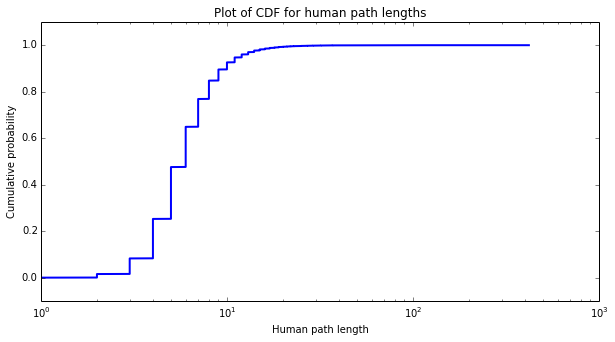
\includegraphics[scale=0.5]{Unknown.png}

From the CDF of the data it is seen that most of the path lengths are less than 30 pages long. Anything larger than this is considered to be an extreme case and is excluded from the histogram plot

\begin{figure}
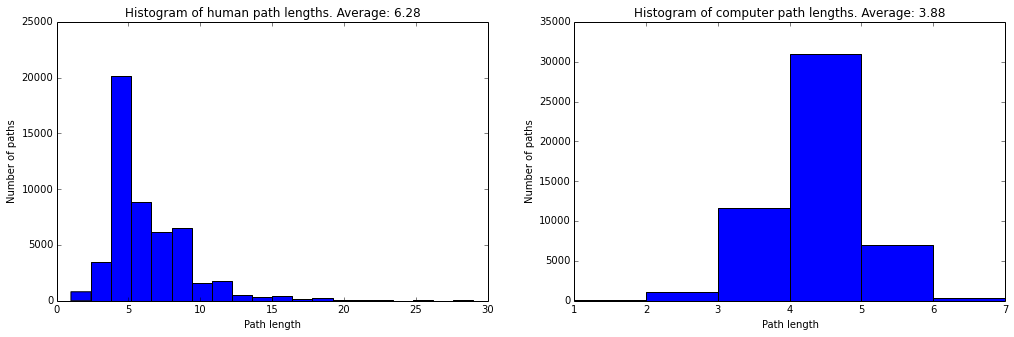
\includegraphics[scale=0.3]{Unknown-2.png}
\caption{Histogram of human path length}
\end{figure}

Shortest path is evaluated considering the most optimum path mathematically. However it doesn't consider the heterogeneity of users and limitations in their knowledge about the subject and their ability to identify the most relevant next link. Many factors such as familiarity of the link or name of the node could also affect clicking of link. These factors, together with the imperfections in users' perception and reasoning capacity, seems to have pushed users away from the shortest path. There are few users who could find the target very closely with the shortest path, but many users took a long route as compared to the shortest path.

From this data, we observe that geographic pages are the most visited and the most used to navigate between different subjects, while scientific pages are used mostly to go to other scientific pages. 

\end{document}